% !TEX root = base.tex 

\chapter{Orientation Dependent Hematite Reactivity}
\label{ch:fe2o3orientation}


\chintro{Bulk and surface orientation have been shown to affect the photochemical
reactivity of semiconductor surfaces. Orientation dependent photochemical reactivity has
been observed for oxide semiconductors. For example, rutile and anatase \ce{TiO2}
microcrystals,\cite{Ohno:2002fn} thin film rutile \ce{TiO2},\cite{Anonymous:YQSV8dnc} and
polycrystalline rutile \ce{TiO2}\cite{Lowekamp:1998ks} have been shown to exhibit
anisotropic activity. Microcrystals of \ce{BaTiO3},\cite{Giocondi:2008ja}
\ce{SrTiO3},\cite{Giocondi:2007fa} and \ce{Sr2Nb2O7}\cite{Giocondi:2008ja} also exhibit
different levels of reactivity for different crystal faces, as does bulk \ce{SrTiO3}
single crystals\cite{Giocondi:2003wc} and polycrystals.\cite{Giocondi:2003wn} Existing
literature on the anisotropic photochemical activity of hematite differentiates between
the basal and prismatic faces of hematite crystals.\cite{Eggleston:2009ic} There are no
reports that differentiate the properties of various prismatic faces and high index
orientations. The results presented in this chapter further our understanding of the
anisotropic photochemical properties of \ce{Fe2O3}, including high index orientations.
In order to accurately decouple effects reported in subsequent chapters from
microstructure, substrate charge, and film orientation on photochemical activity, the
dependence of photochemical activity on crystallite orientation was examined.  These
results provide the baseline information for interpretation of other photochemical
experiments on \ce{Fe2O3} presented in this document.}



\section{Experimental Details}
\label{sec:ch9experimental}


Electron backscatter diffraction (\abbr{EBSD}) was used to determine grain orientations of
a polycrystalline \textalpha-\ce{Fe2O3} pellet. By using a polycrystalline sample, a wide
variety of orientations, covering the entire range of the standard stereographic triangle
representing all possible surface orientations, can be examined in a single experimental
run. 

A polished \ce{Fe2O3} pellet was prepared as described in Chapter~\ref{ch:experimental}.
To promote grain growth, the pellet was sintered for at \SI{1200}{\degreeCelsius} for
\SI{48}{\hour} in air, rather than the sintering procedure in Chapter
\ref{ch:experimental}. No other changes from the established sample synthesis procedure
were made. An orientation map of the sample was obtained using electron backscatter
diffraction. Backscatter patterns were of consistent high quality over the entire examined
area. Acquisition was performed under high vacuum with an accelerating voltage of
\SI{20}{\kilo\volt}. 

Photochemical activity was measured using the established reaction of the reduction of
aqueous silver ions to neutral solid silver. Reactions were carried out under illumination
from a narrow spectrum blue \abbr{LED} (Philips Lumiled, \textlambda$_\text{peak}$ =
\SI{470}{\nano\meter} and broad spectrum Xe arc lamp (\SI{150}{\watt}, Newport, Bozeman,
\abbr{MT}). The reaction time was varied depending on the light source and characterization
technique. Table \ref{tab:reactiontimes} lists the reaction times used for this work.
\begin{table}
\begin{center}
  \begin{tabular}{lrr}

   Characterization Method & Xe Lamp  & Blue \abbr{LED}  \\
  
   \cmidrule(lr){1-1}
   \cmidrule(lr){2-2}
   \cmidrule(lr){3-3}
   
   Optical & \SI{5}{\minute} & \SI{15}{\minute} \\
   \abbr{SEM} & \SI{5}{\minute} &  --\\
   \abbr{AFM} & \SI{30}{\second} & -- \\

\end{tabular}
\end{center}
  \caption[Reaction times for photochemical experiments]{Reaction times for photochemical
experiments presented in this chapter. Reaction time varied depending on illumination
source and observational technique. These times were selected to provide optimal imaging
conditions for each technique.}
  \label{tab:reactiontimes}
\end{table}
Reaction times were chosen to provide the best level of reaction product for the
respective observation technique. For example, for optical microscopy, a large amount of
reaction product will provide maximum contrast, but for atomic force microscopy, too many
solid silver particles on the surface will cause difficulty in accurately measuring the
topography of the surface. 

The surface of the sample was examined before and after photochemical reaction with
scanning electron (\abbr{SEM}), atomic force (\abbr{AFM}), and Kelvin probe force
(\abbr{KFM}) microscopy. Scanning electron microscopy allow for rapid analysis of many
grains simultaneously, but grains that have low (but nonzero) levels of reactivity may be
missed. Atomic force measurements provide extremely accurate measures of reactivity,
including low and moderate levels of reaction product, but are comparatively time
consuming and difficult to obtain. All methods were used to verify the presence of
reaction product on a wide range of crystallite orientations. Kelvin probe force
microscopy was used to examine the local surface potential of reactive and nonreactive
grains.

Scanning electron microscopy was performed using a Quanta 200 \abbr{FE-SEM} 
(\abbr{FEI} Company, Mahwah,
\abbr{NJ}) with an accelerating voltage of \SI{5.0}{\kilo\volt}. \abbr{AFM} images were
collected using an \abbr{NT}egra \abbr{AFM} (\abbr{NT-MDT}, Moscow) using standard
semicontact techniques. \abbr{KFM} images were obtained using a Solver\abbr{NEXT}
\abbr{AFM} (\abbr{NT-MDT}).


\section{Results}
\label{sec:ch9results}


\subsection{Scanning Electron Microscopy}
\label{subsec:ch9sem}


\figureref{semimages} shows \abbr{SEM} micrographs of the \ce{Fe2O3} surface after
reaction.
\begin{figure}
	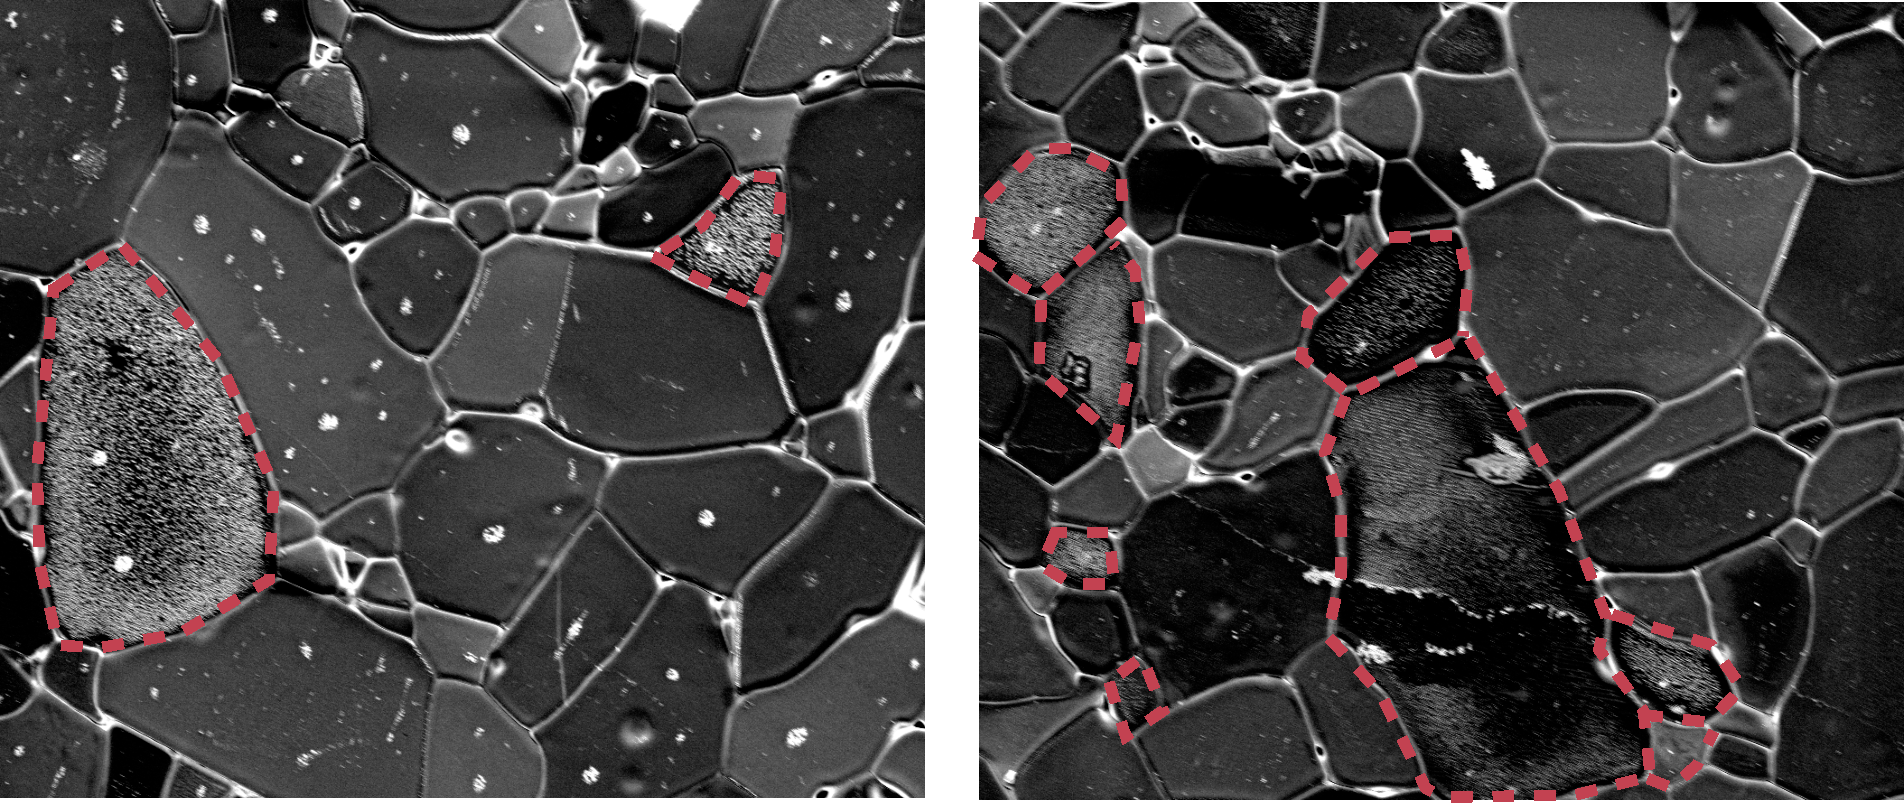
\includegraphics[width=\textwidth]{semimages.pdf}
	\caption[Representative \abbr{SEM} micrographs after photochemical reaction]{%
		Representative \abbr{SEM} micrographs of \ce{Fe2O3} polycrystals taken after
photochemical reaction showing reactive and nonreactive grains. Grains were identified as 
		reactive by manual inspection. Reaction product appears as bright white areas
within a grain. Reactive 
		grains are outlined in red in these micrographs. Other sources of white contrast
include grain boundaries and 
		pores.}
	\label{fig:semimages}
\end{figure}
Reaction product appears as bright areas within grains in the \abbr{SEM} micrographs.
Additional white contrast appears in the form of grain boundaries and pores, presumably
arising from charging of the weakly conducting sample. Reactive grains are outlined on the
micrographs in \figureref{semimages}. Grains were manually identified as reactive or
nonreactive. \abbr{SEM} images were collected to cover a large area of the sample. The
images in \figureref{semimages} are representative of all collected micrographs.

\figureref{ebsdmapsem} shows the complete inverse pole map collected via \abbr{EBSD} and a
subset of the map corresponding to the grains marked as reactive during \abbr{SEM}
observation.
\begin{figure}
	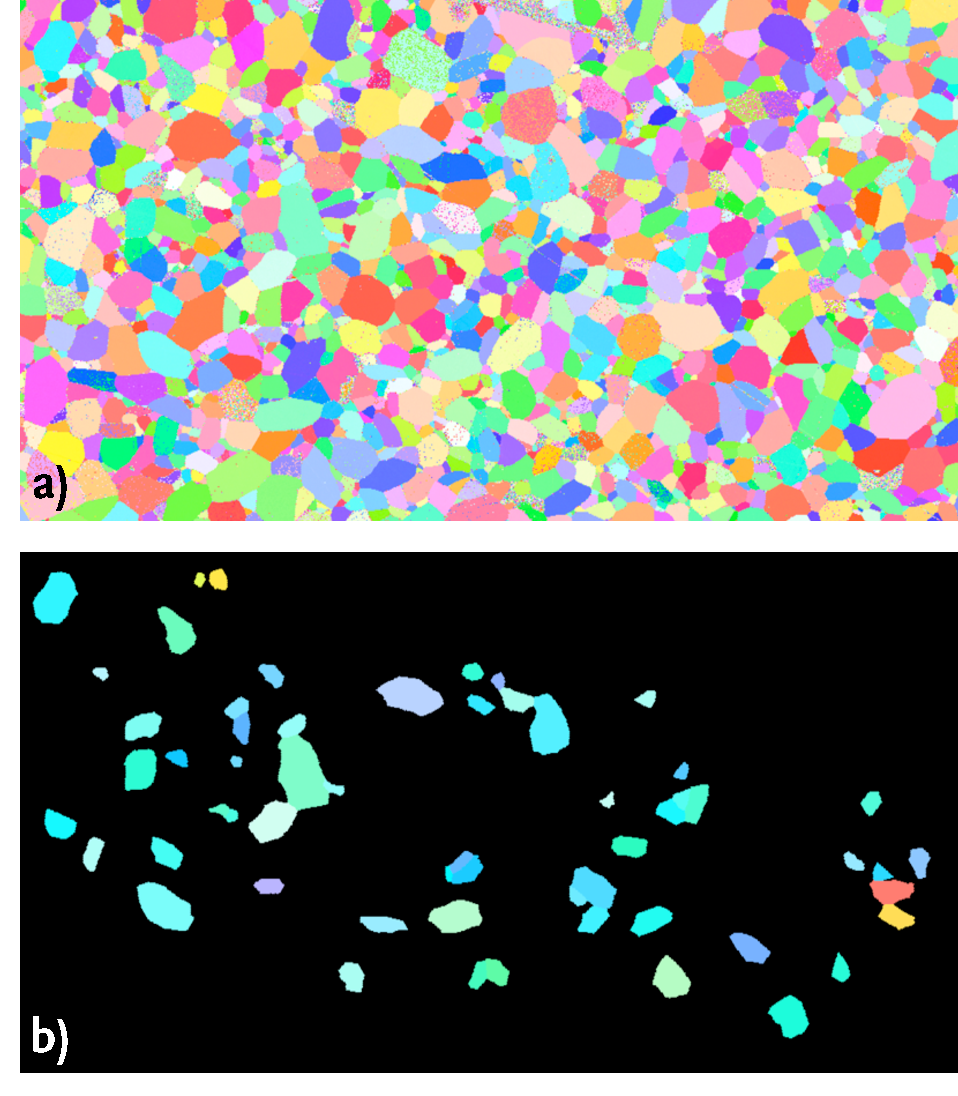
\includegraphics[width=\textwidth]{ebsdmapssem.pdf} %maybe make these side by side and
%then have a wholewidth figure
	\caption[Inverse pole maps of \ce{Fe2O3} surface]{%
		Electron backscatter diffraction inverse pole maps of the 
		observed area of the \ce{Fe2O3} surface. (a) Map including 
		all grains in the observed area. (b) The subset of grains 
		identified as reactive during \abbr{SEM} analysis of the surface 
		after photochemical reaction with \ce{AgNO3}. These grains 
		correspond to the points on the standard stereographic triangle 
		in \figureref{semtriangle}. The similar color of these 
		grains in the inverse pole map suggests that the majority 
		of active grains are similarly oriented. }
\label{fig:ebsdmapsem}
\end{figure}
\begin{figure}
	\centerline{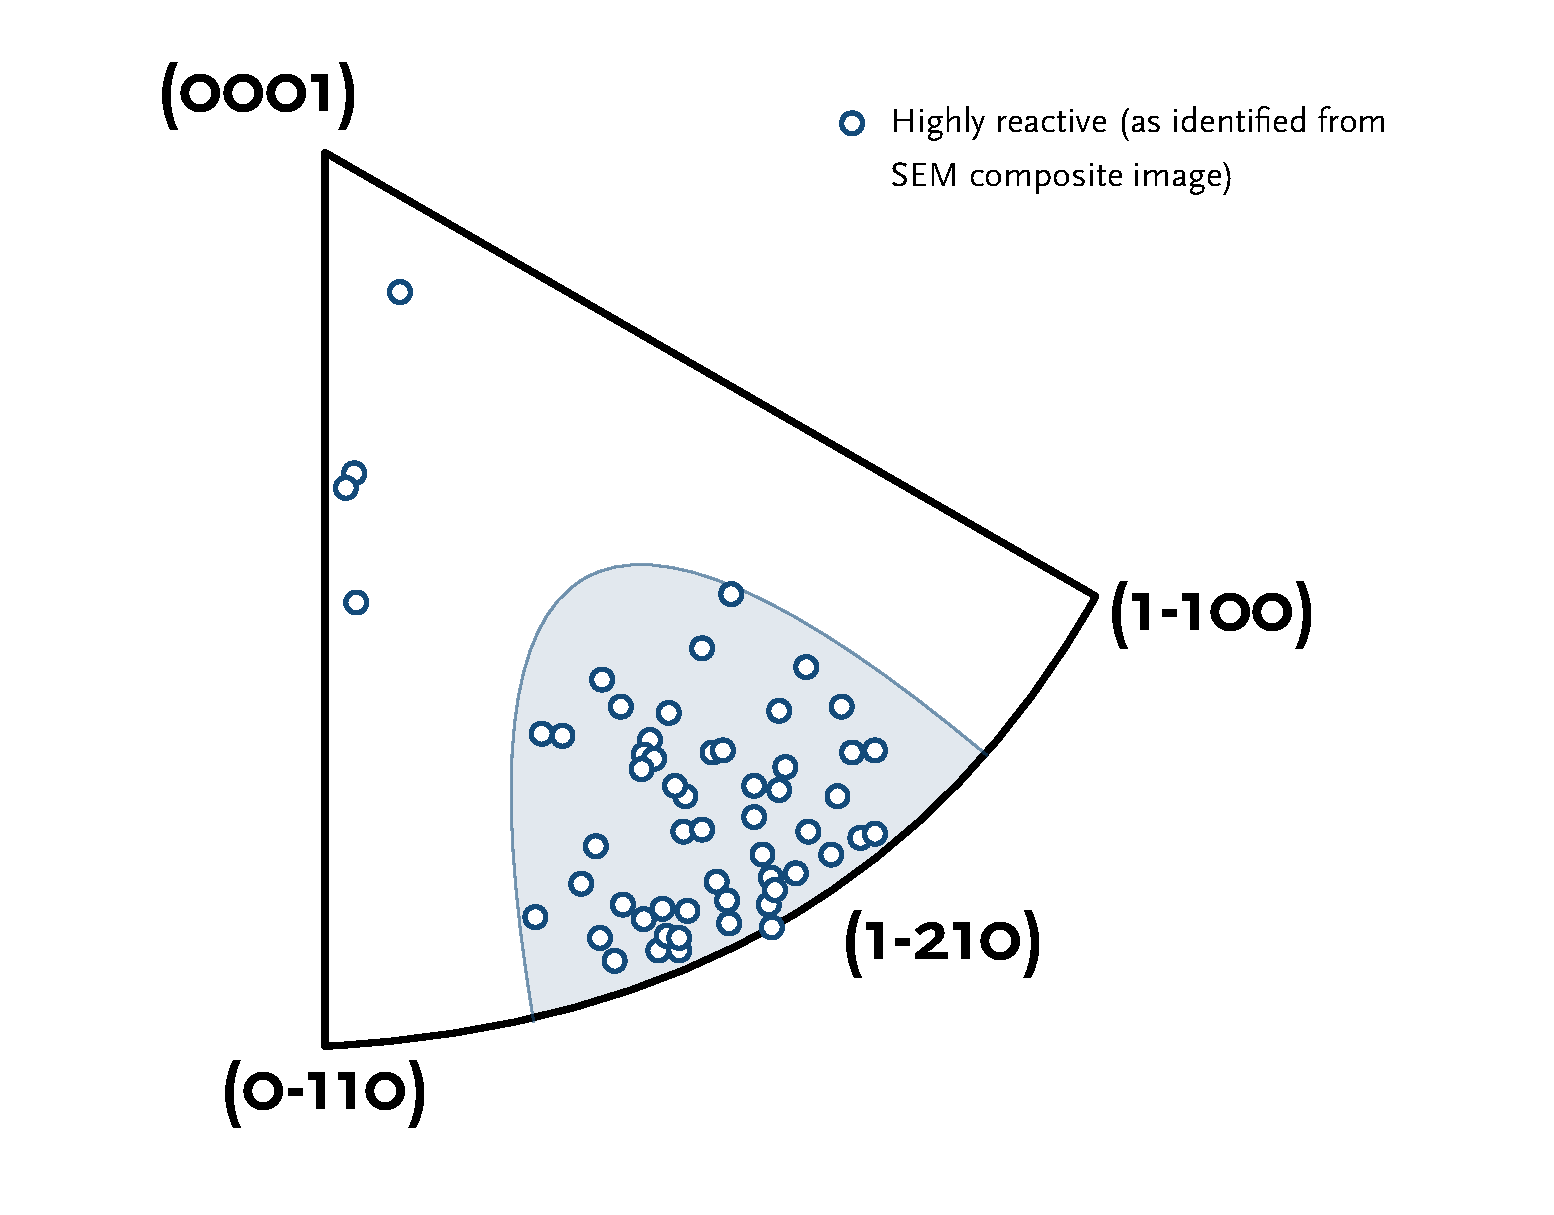
\includegraphics[width=0.6\textwidth]{semtriangle.pdf}}
		\caption[Reactive grains from \figureref{ebsdmapsem}]{%
			Reactive grains from \figureref{ebsdmapsem} plotted on 
			the standard stereographic triangle for hexagonal crystals. Each 
			point in the triangle represents the orientation of a grain 
			identified as reactive. The blue shaded area outlines the cluster 
			of highly reactive grains near the (1\={2}10) orientation. With 
			four exceptions, all observed reactive grains were oriented near 
			this orientation.}
	\label{fig:semtriangle}
\end{figure}
The grains identified as reactive generally fall within a similar color range, suggesting
strong orientation effects on photochemical activity. The difference between reactive and
nonreactive grains was very obvious for most grains; reactive grains were generally
completely or mostly covered with bright reaction product, while nonreactive grains were
completely devoid of any contrast from solid silver on the surface. The points identified
as reactive were plotted on the standard stereographic triangle for hexagonal crystal
systems, presented in \figureref{semtriangle}. This triangle represents the entire
possible set of orientations. Points on the triangle represent observed reactive grains.
With four exceptions, all points lie within about 10-15\degree{} from the (1\={2}10) pole.


\subsection{Atomic Force Microscopy}
\label{subsec:ch9afm}


To verify the rapid but imprecise classifications of reactivity obtained via
scanning electron microscopy, the reacted sample was examined using atomic force
microscopy. The results from the \abbr{SEM} images were used to determine appropriate
locations for study. To increase the amount of data obtained through \abbr{AFM}, scan
locations were selected that contained multiple grains, including both reactive and
nonreactive grains as identified in \abbr{SEM} images. Six scan areas were selected,
comprising a total of approximately 60 grains of varying orientation.
\figureref{fe2o3afmmap} shows an inverse pole map displaying which grains were observed
using \abbr{AFM}.
\begin{figure}
	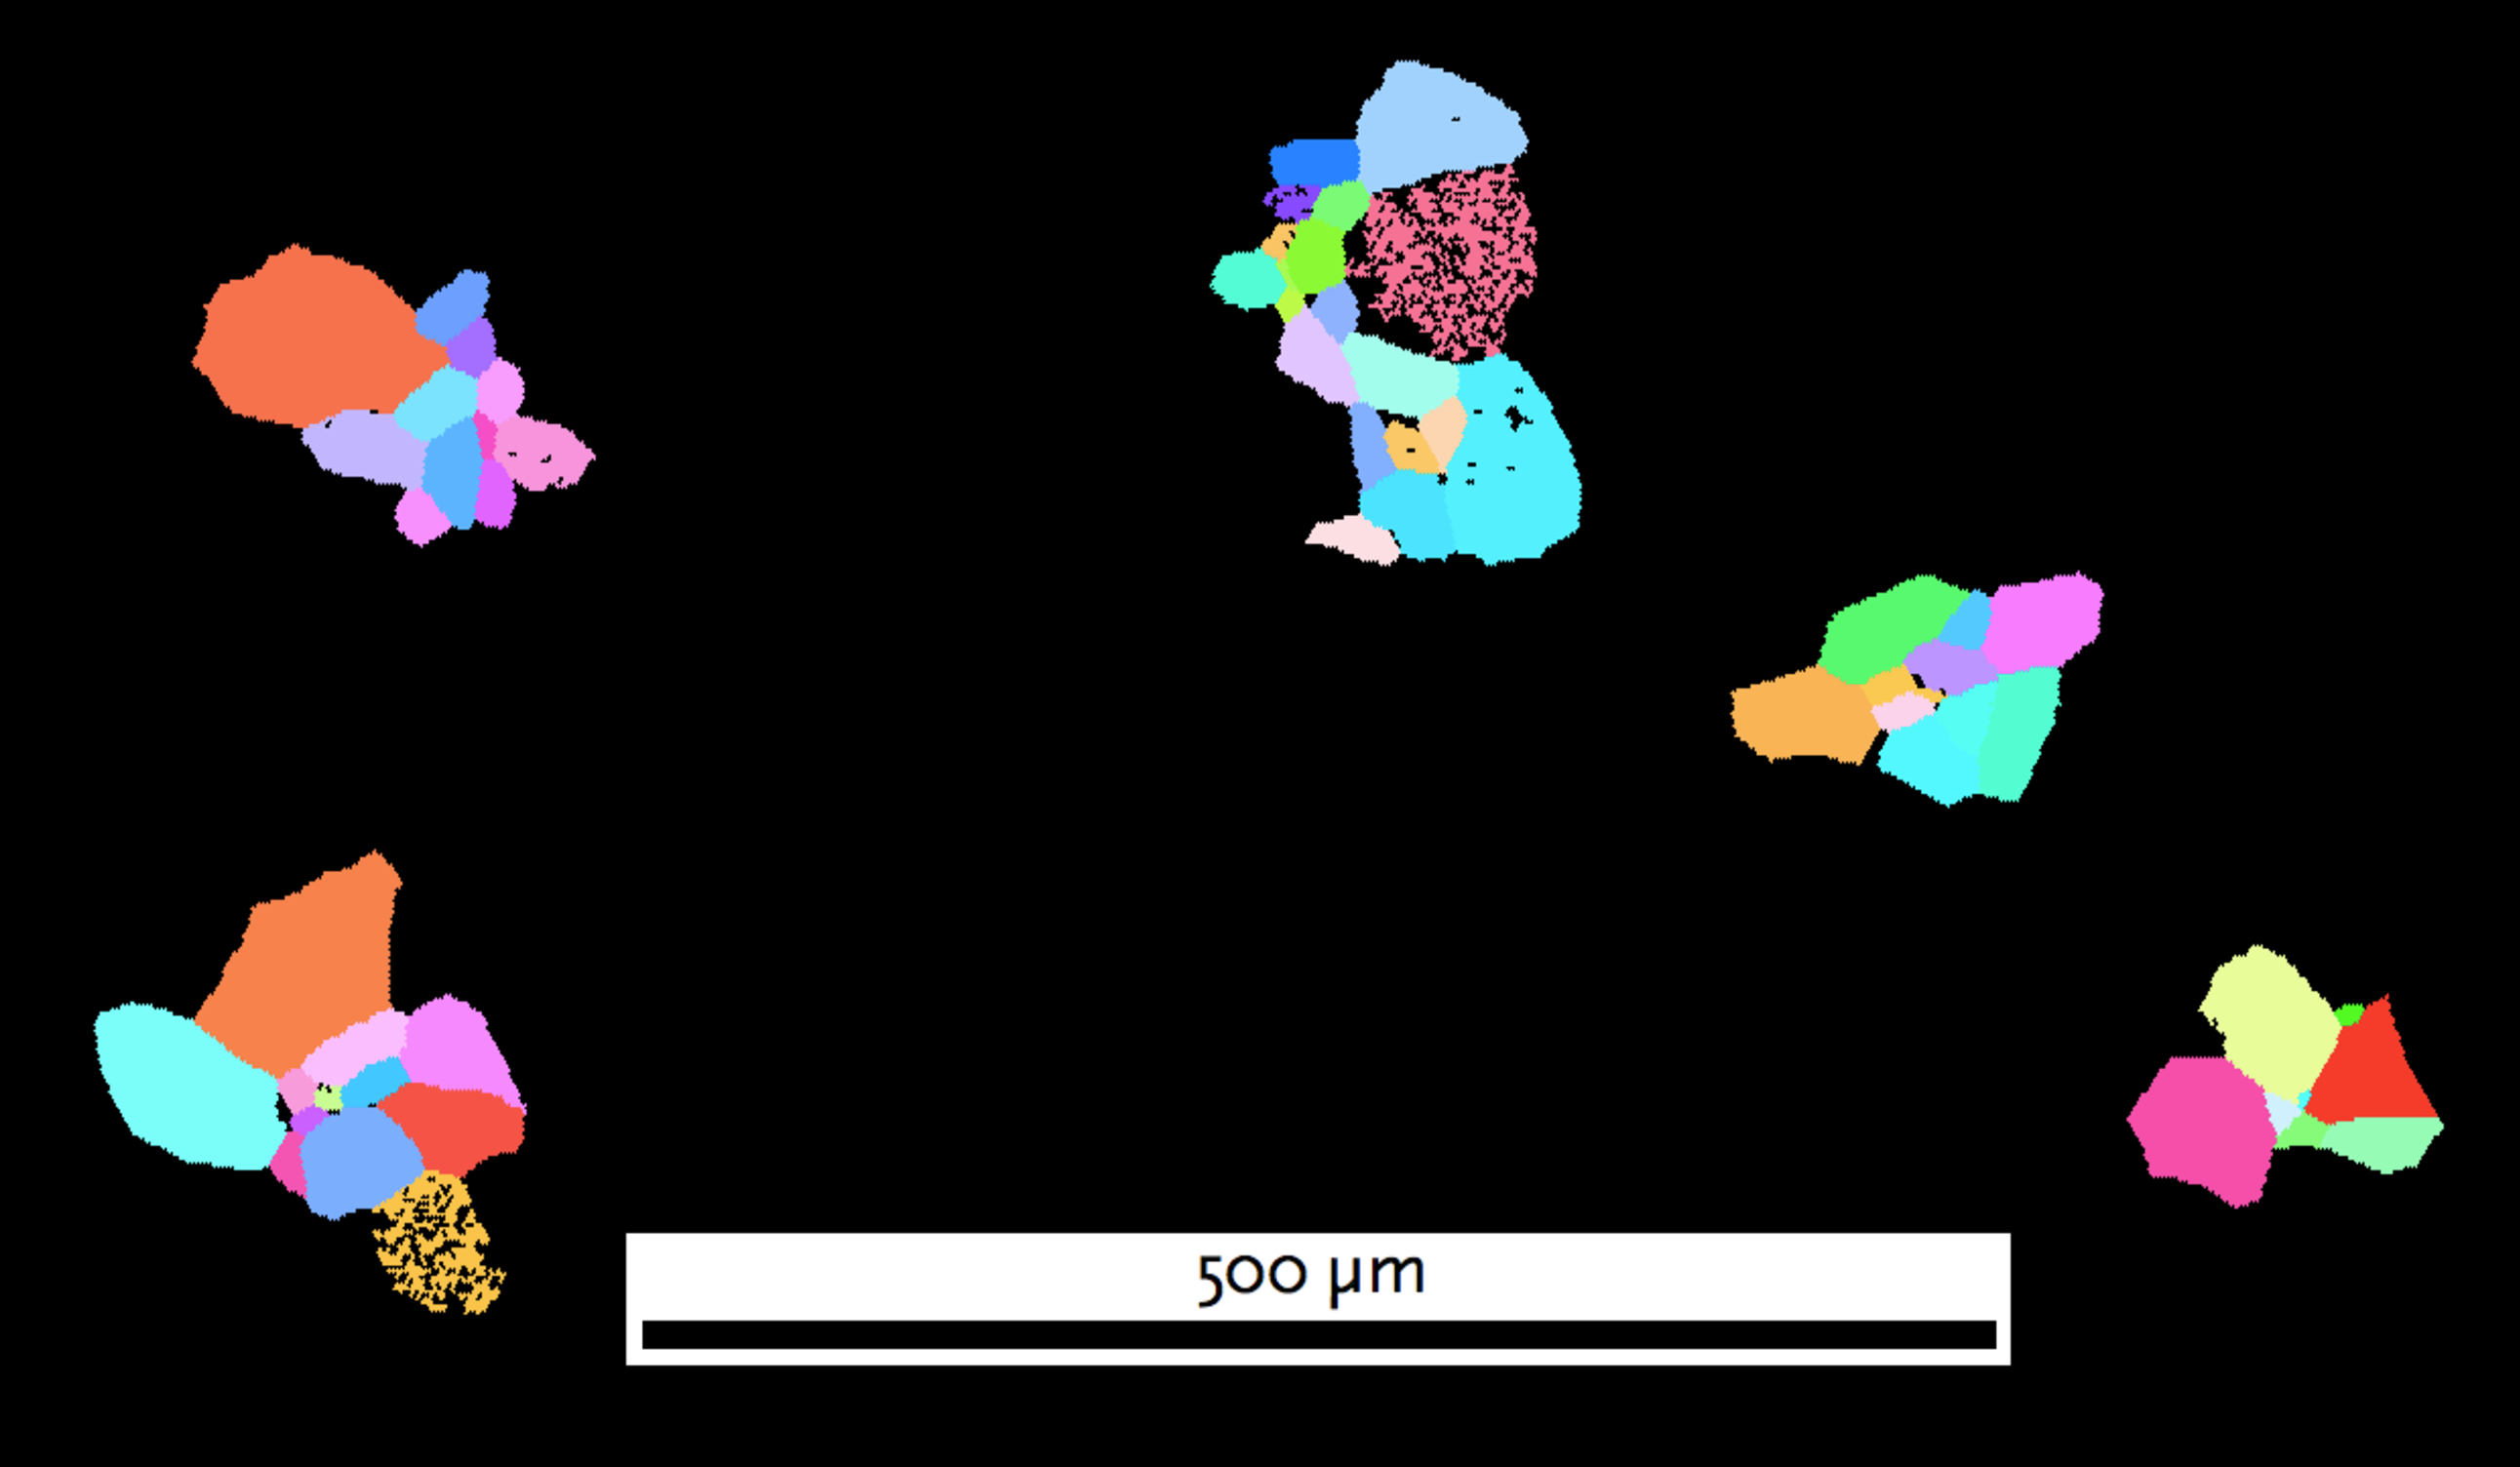
\includegraphics[width=\textwidth]{fe2o3afmmap.pdf}
	\caption[Inverse pole map of grains observed using \abbr{AFM}.]{%
		Inverse pole map showing the portion of grains observed using atomic force
microscopy. This source data for this 
		figure is the same as for \figureref{ebsdmapsem}.}
	\label{fig:fe2o3afmmap}
\end{figure}

Figures \ref{fig:fe2o3afmscans}(a)-(c) show the representative \abbr{AFM} scans of the
sample surface after reaction under illumination from a Xe arc lamp for \SI{30}{\second}.
All scans have dimensions of \SI{50}{\micro\meter} \texttimes{} \SI{50}{\micro\meter}.
Three levels of reactivity were manually assigned to each grain. Grains that were entirely
covered in reaction product were labelled highly reactive. In \figureref{fe2o3afmscans},
these grains are outlined in blue. Grains with partial reactivity, such as reactive areas
or grain edges were labeled moderately reactive. \figureref{fe2o3afmscans}(c) contains a
moderately reactive grain, outlined in green.
\begin{figure}[b]
	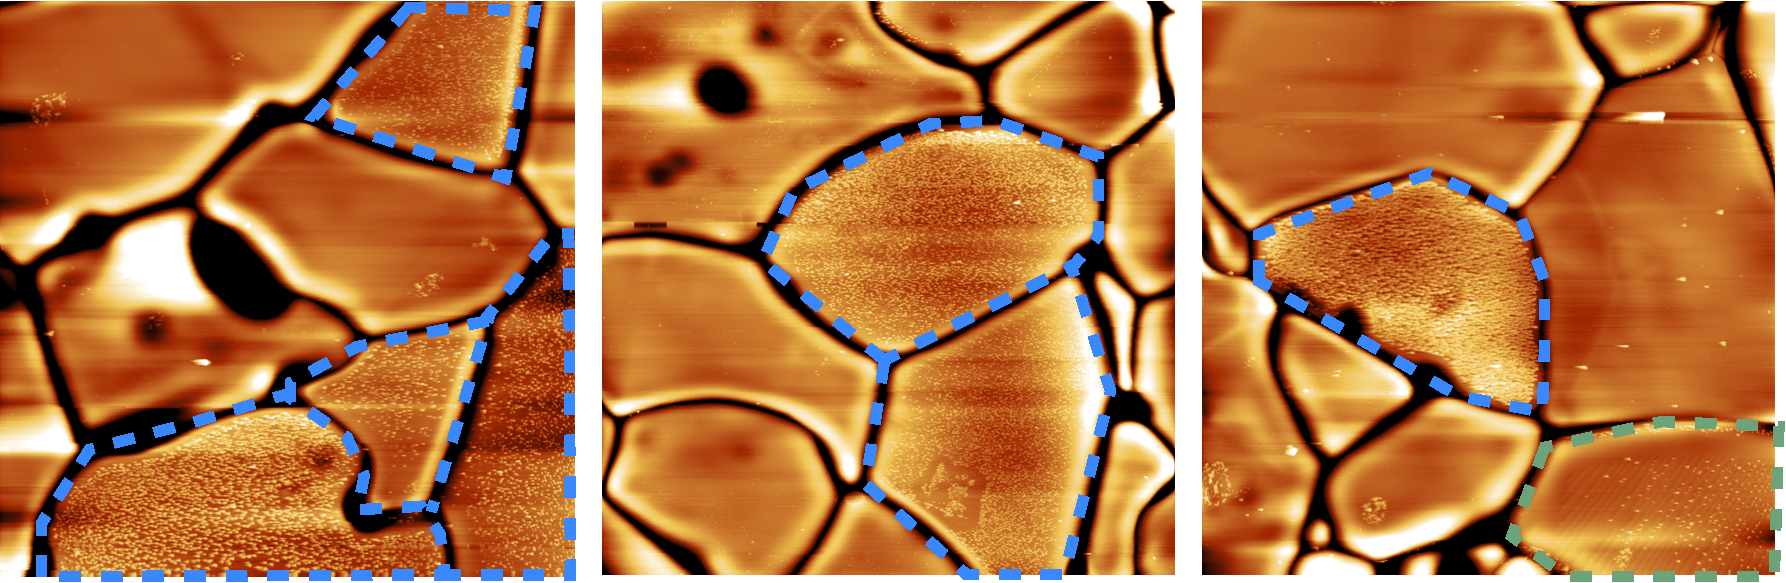
\includegraphics[width=\textwidth]{fe2o3afmscans.pdf}
	\caption[Representative \abbr{AFM} scans of three examined areas]{%
		Representative \abbr{AFM} scans of three examined areas. Highly reactive grains
are outline in blue. 
		Moderately reactive grains are outlined in green. These scans are representative
of all scans 
		obtained via \abbr{AFM}. The size of each image is \SI{50}{\micro\meter}
\texttimes{} \SI{50}{\micro\meter}.}
	\label{fig:fe2o3afmscans}
\end{figure} 

\begin{figure}
	\centerline{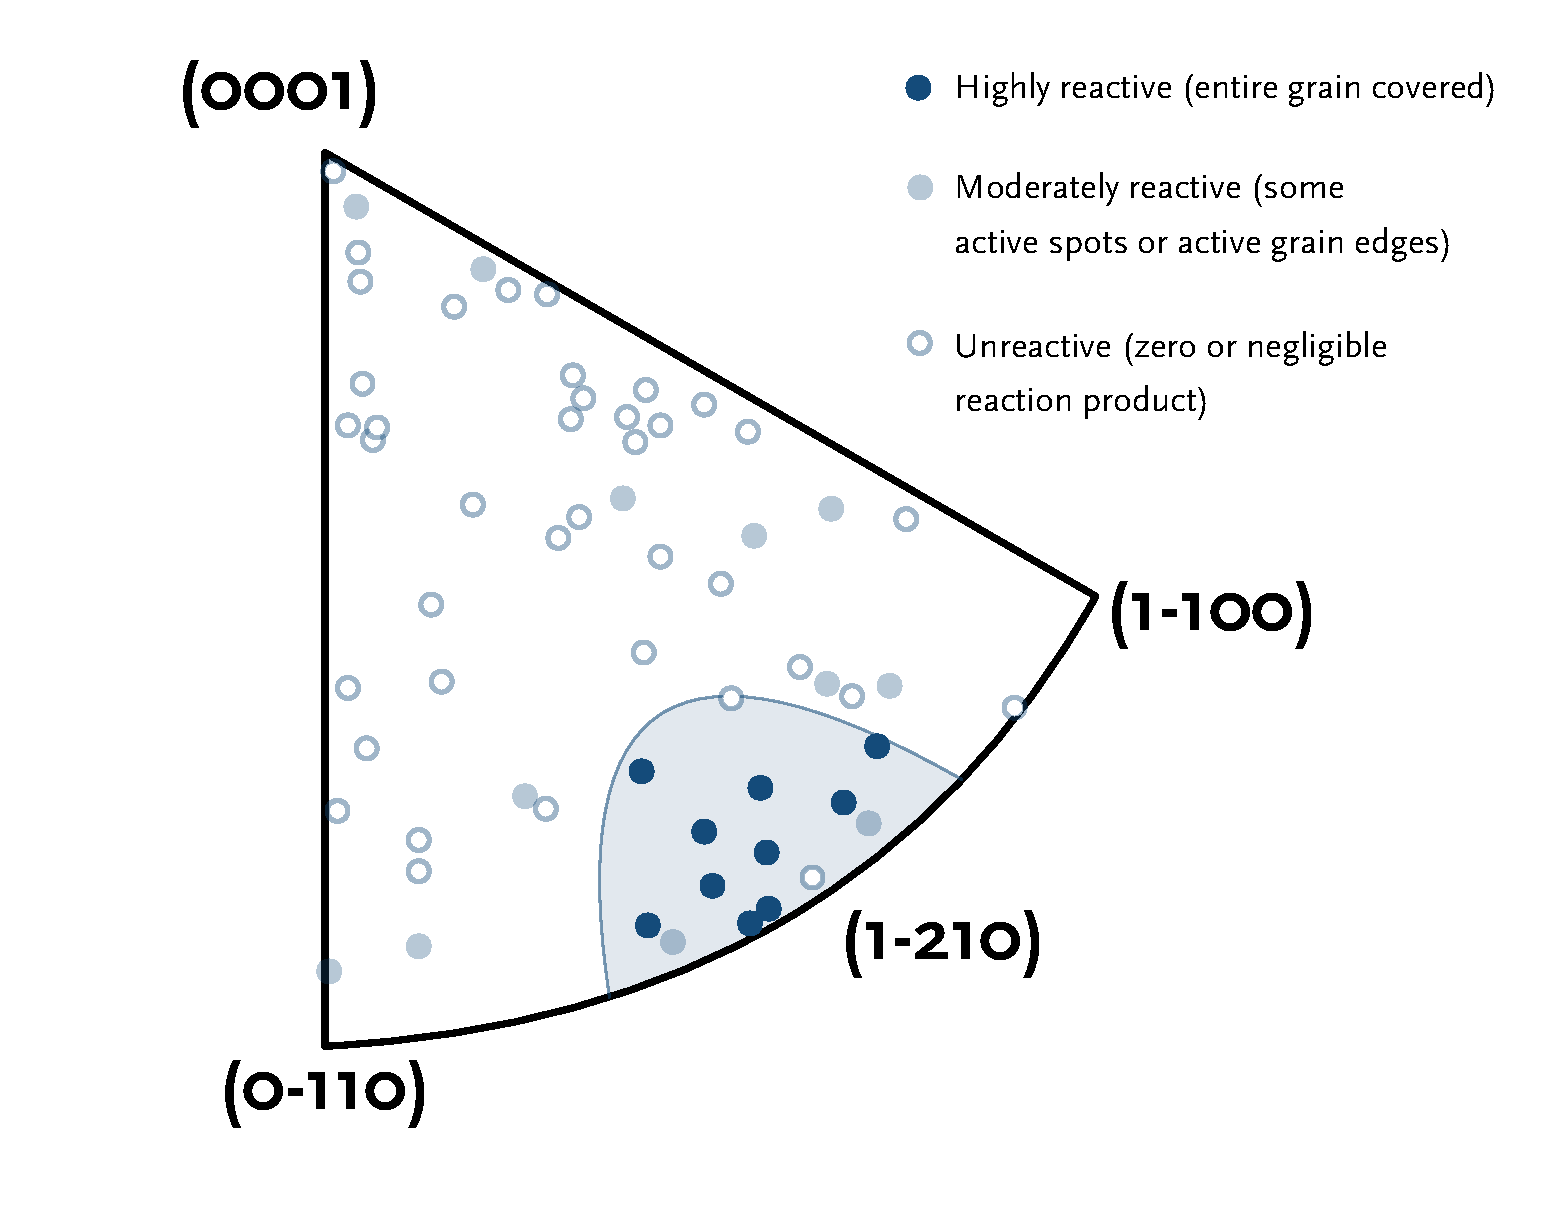
\includegraphics[width=0.6\textwidth]{afmtriangle.pdf}}
		\caption[Reactive grains from \figureref{fe2o3afmmap}]{%
			All grains from \figureref{fe2o3afmscans} plotted on the 
			hexagonal standard sterographic triangle. Highly reactive grains 
			are dark blue, moderately reactive grains are light blue, and 
			nonreactive grains are open circles. All highly reactive grains 
			are located near the (1\={2}10) orientation.}
	\label{fig:afmtriangle}	
\end{figure}
After classifying all grains contained in the full set of \abbr{AFM} scans, each point was
plotted on the standard stereographic triangle for hexagonal crystal systems, similar to
\figureref{semtriangle}. The resulting triangle for \abbr{AFM} classification is depicted
in \figureref{afmtriangle}. As compared to \figureref{semtriangle}, the including of
nonreactive and moderately reactive points provides additional information. Similar to the
triangle constructed for the \abbr{SEM} results, all highly reactive grains are clustered
near the (1\={2}10) orientation. However, some moderately reactive or nonreactive grains
are observed in this area as well. The data presented here suggest that not all grains
oriented near (1\={2}10) are highly reactive. At the same time, no highly reactive grains
are observed far away from the (1\={2}10) orientation. In summary, the data in this figure
suggests that a reactive grain is likely near the (1\={2}10) orientation, but that a grain
having this orientation is not a guaranteed to exhibit high reactivity. It is proposed
that this is a result of the symmetry of hematite. While not unusual to treat hematite as
hexagonal, it is actually trigonal. For trigonal crystals, there are only three
indistinguishable (1\={2}10) surfaces, rather than six. This difference may explain why on
a subset of grains near the hexagonal (1\={2}10) orientation are reactive.


\subsection{Kelvin Probe Force Microscopy}
\label{subsec:ch9kfm}


The local surface potential of reactive and nonreactive grains was obtained using Kelvin
probe force microscopy (\abbr{KFM}). \abbr{KFM} is a two-pass semicontact mode technique.
The first pass acquires the sample topography. During the second pass, the tip is lifted a
user-defined distance above the sample surface. Using the topography data acquired during
the first pass, the tip is kept at this same distance from the surface during the entire
pass. An ac-bias is applied to the tip, causing it to oscillate. A dc-bias is then applied
until the oscillations cease; this dc-bias corresponds to the local potential of the
sample surface.

\figureref{fe2o3kfmscans} shows representative \abbr{KFM} scans of the \ce{Fe2O3} surface.
\begin{figure}
	\includegraphics[width=\textwidth]{fe2o3kfmscans.pdf}
	\caption[Two representative \abbr{KFM} scans]{%
		Two representative \abbr{KFM} scans. Each row shows an optical micrograph of the
scan area, 
		from which grain reactivity was determined. Also depicted in each row are the simultaneously 
		acquired topography and surface potential micrographs. Bright areas in the surface
		potential image correspond to higher surface potential. The topography image is
		included to demonstrate that contrast in the surface potential image is not an artifact of
		topography. The surface potential shows some features not present in topography and also 
		omits features such as certain grain boundaries.}
	\label{fig:fe2o3kfmscans}
\end{figure}
Scan areas were selected to include both reactive and nonreactive grains, as determined in
\sectionref{subsec:ch9sem} and \sectionref{subsec:ch9afm}. Five total scans were obtained,
comprising 29 identified grains. The simultaneously acquired topography and surface
potential images are shown. Brighter contrast in the surface potential image represents
higher surface potential. Consistently across all scans, reactive grains had a higher
surface potential than nonreactive grains. \figureref{fe2o3kfmplots} plots the surface
potentials of the grains within each scan, as well as one plot of all combined data. The
surface potential for each grain was calculated using the average potential with a 10
\texttimes{} 10 pixel box at the center of each grain. Previously obtained optical images,
also included in \figureref{fe2o3kfmscans} were used to categorize each grain as reactive
or nonreactive. This classification is reflected in the plots in
\figureref{fe2o3kfmplots}.
\begin{figure}
\centering
$\begin{array}{cc}
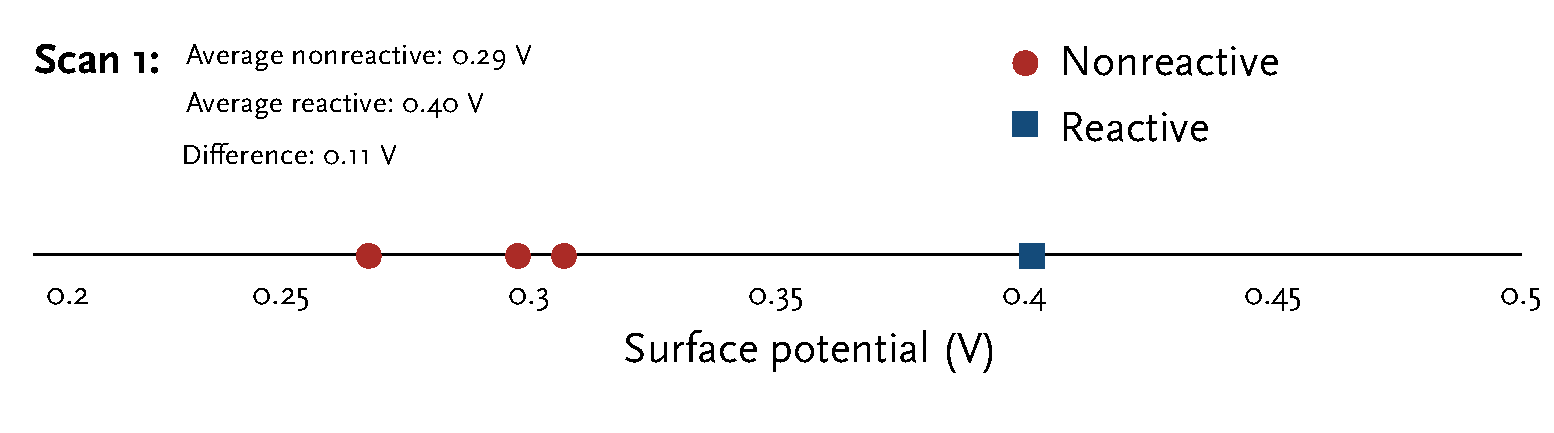
\includegraphics[width=0.8\textwidth]{Scan1.pdf} \\ 
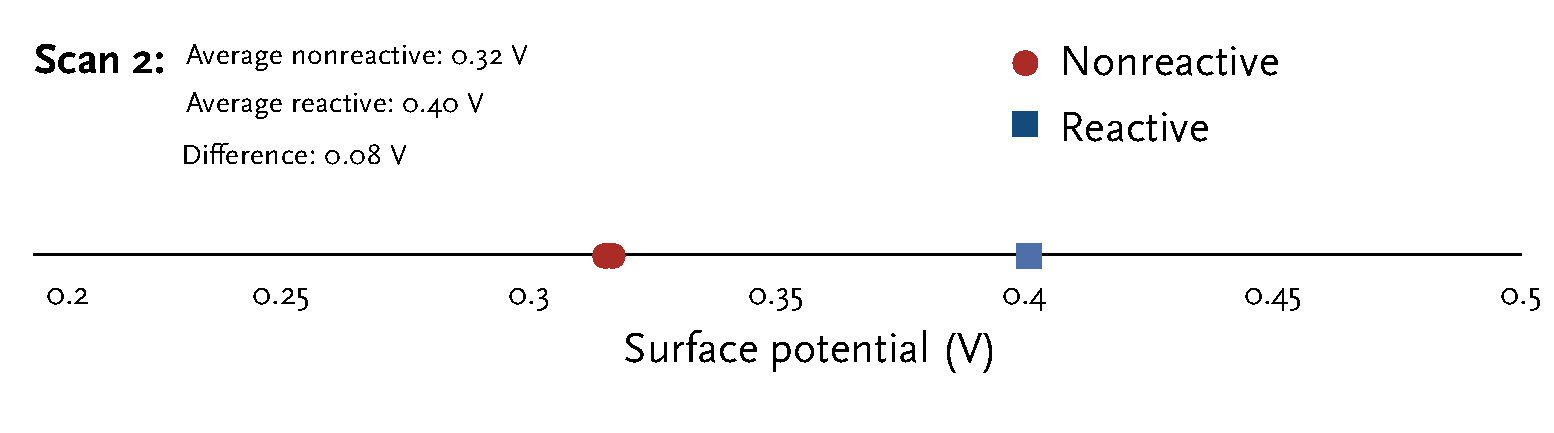
\includegraphics[width=0.8\textwidth]{Scan2.pdf} \\ 
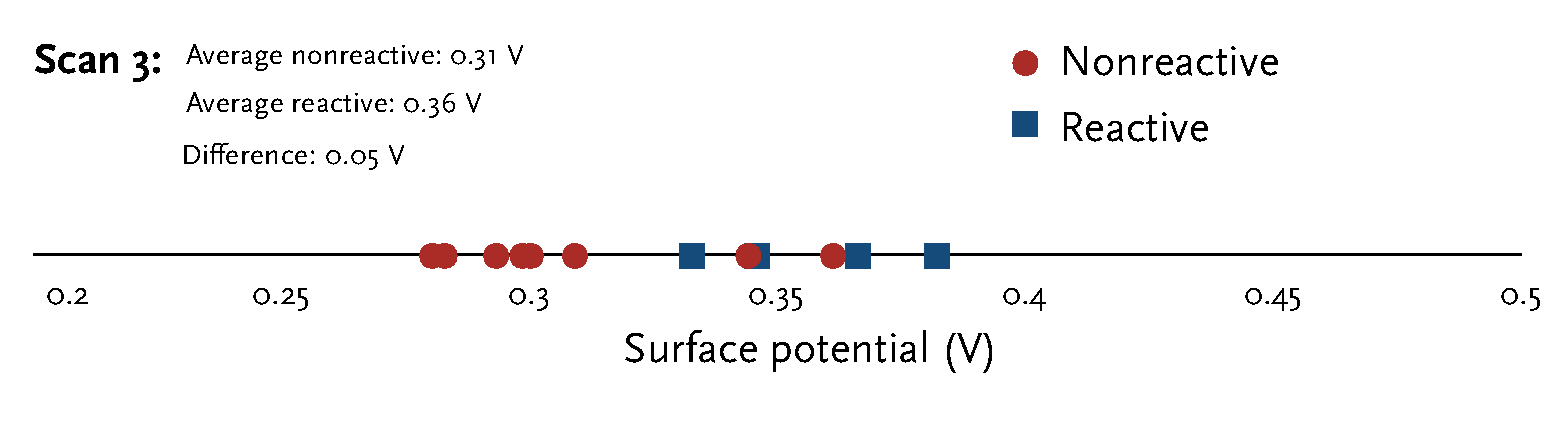
\includegraphics[width=0.8\textwidth]{Scan3.pdf} \\ 
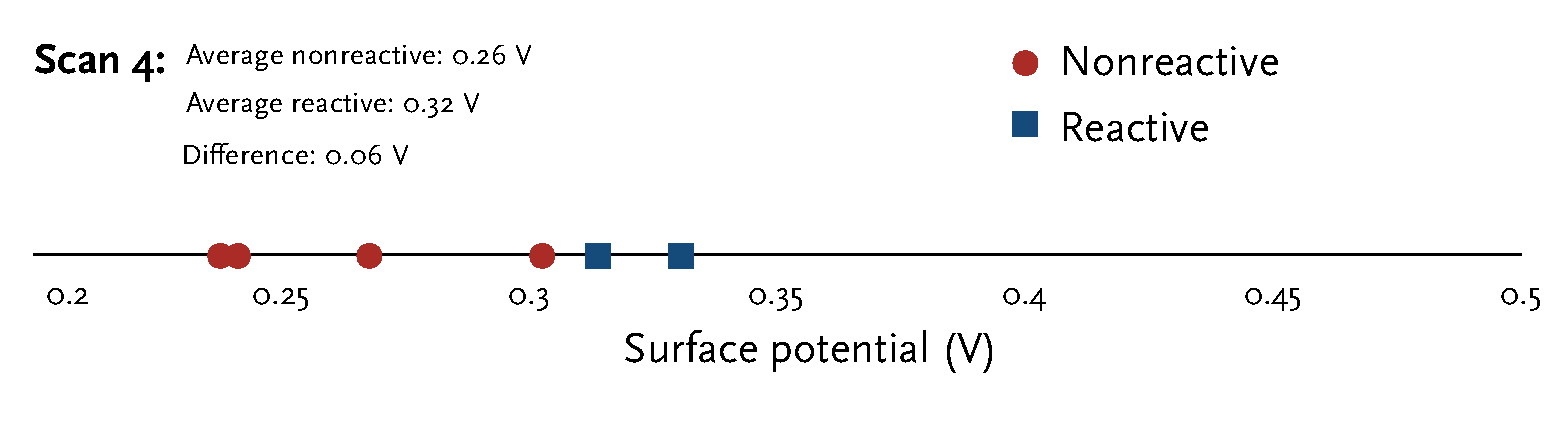
\includegraphics[width=0.8\textwidth]{Scan4.pdf} \\ 
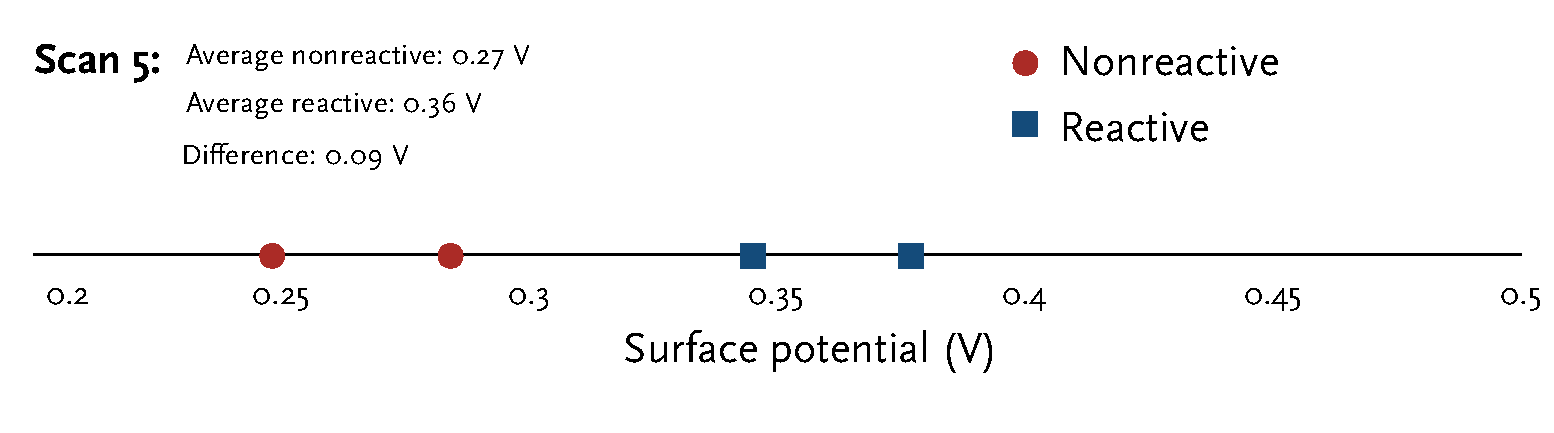
\includegraphics[width=0.8\textwidth]{Scan5.pdf} \\ 
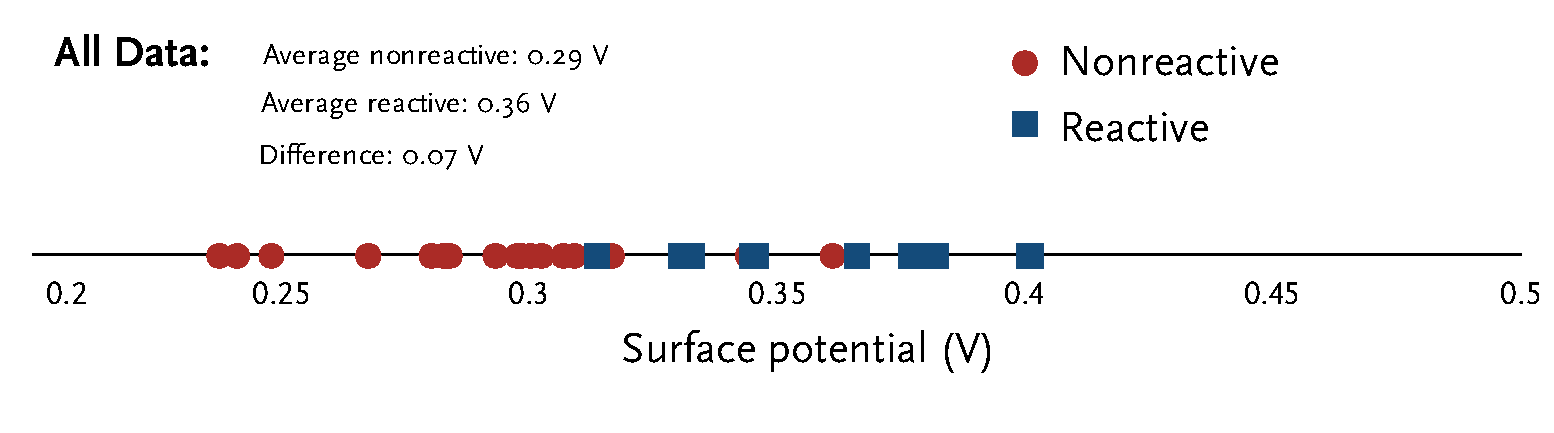
\includegraphics[width=0.8\textwidth]{AllData.pdf}
\end{array}$
\caption[Average surface potential for each grain]{Plots of the average surface potential
for each grain within each scan, as well as the amalgamated data from all scans. Reactive
grains appear as blue boxes and nonreactive grains appear as read circles on the plots.
With two exceptions, the grains with the highest surface potential in each scan were the
most reactive. The average difference in surface potential between reactive and
nonreactive grains was \SI{70}{\milli\volt}.}
\label{fig:fe2o3kfmplots}
\end{figure}
On average, reactive grains had a surface potential \SI{70}{\milli\volt} higher than
nonreactive grains. The correlation between highly reactive grains and a higher surface
potential was clear for all scans. With only a few exceptions, the grains with the highest
surface potential within each scan were the reactive grains.

\section{Discussion}\label{sec:ch9discussion}

The data show that hematite polycrystals exhibit extremely anisotropic photochemical
activity. Grains oriented near the (1\={2}10) orientation are significantly more reactive
than other grains at the surface. This remains true both under ultraviolet and visible
light illumination. \abbr{AFM} images suggest that this is unrelated to the presence of
facets at the surface. Both faceted and nonfaceted grains were observed to be reactive or
nonreactive.

Earlier studies of photochemical anisotropic behavior of oxide polycrystals have
attributed the effect to both surface and bulk properties. For example, Giocondi et
al.\cite{Giocondi:2007fa} attributed the photochemical activity of \ce{SrTiO3}
polycrystals to differences in the energy levels of the band dispersion. The authors
suggested that higher rates of reactivity were the result of an increased generation of
carriers with momentum along certain crystal directions. On the other hand, Lowekamp et
al.\cite{Lowekamp:1998ks} suggest that the increased reactivity of \ce{TiO2} polycrystals
arises from the presence of highly active surface planes, rather than from a bulk
property. Because of the lack of conclusive evidence supporting the bulk or surface cause
of anisotropic photochemical reactivity for oxide polycrystals, both possibilities will be
examined here.

For hexagonal crystal systems, studies of anisotropic properties often focus on property
differences between basal and prismatic planes. The basal plane is defined as the plane
perpendicular to the c-axis of the unit cell. The prismatic planes are the set of planes
parallel to the c-axis, intersecting the a-axis directions of the unit cell. For example,
in corundum-type materials, which includes \textalpha-\ce{Fe2O3}, the structure consists
of close-packed oxygen planes stacked along the c-axis, with \ce{Fe^{3+}} ions filling two
thirds of the interstitial sites. As a result, electron travel within the basal plane
occurs within planes of iron ions, while travel perpendicular to the plane results in
traversing layers basal layers of oxygen ions.\cite{Iordanova:2005ha} As a result,
anisotropic electrical properties have been observed when comparing these
directions.\cite{Benjelloun:1984cq}

For \ce{Fe2O3}, differences in electron conductivity between the basal plane and the
prismatic planes are observed. Conductivity along the c-axis direction in \ce{Fe2O3} is
lower than along perpendicualr directions.\cite{Huda:2010kx,Iordanova:2005ha}
Photochemical experiments determined that the onset of photocurrent for hematite basal
planes is different than that of prismatic planes.\cite{Eggleston:2009ic} Prismatic faces
of the crystal showed an earlier onset of photocurrent than basal planes. That study only
differentiated between properties of the basal plane and the prismatic planes, and did not
study differences in properties between the prismatic faces. The work presented here shows
a strong difference in photochemical properties not only between the basal and prismatic
orientations, but also determined that one prismatic orientation is significantly more
reactive than the others. 

\begin{figure}
\begin{center}
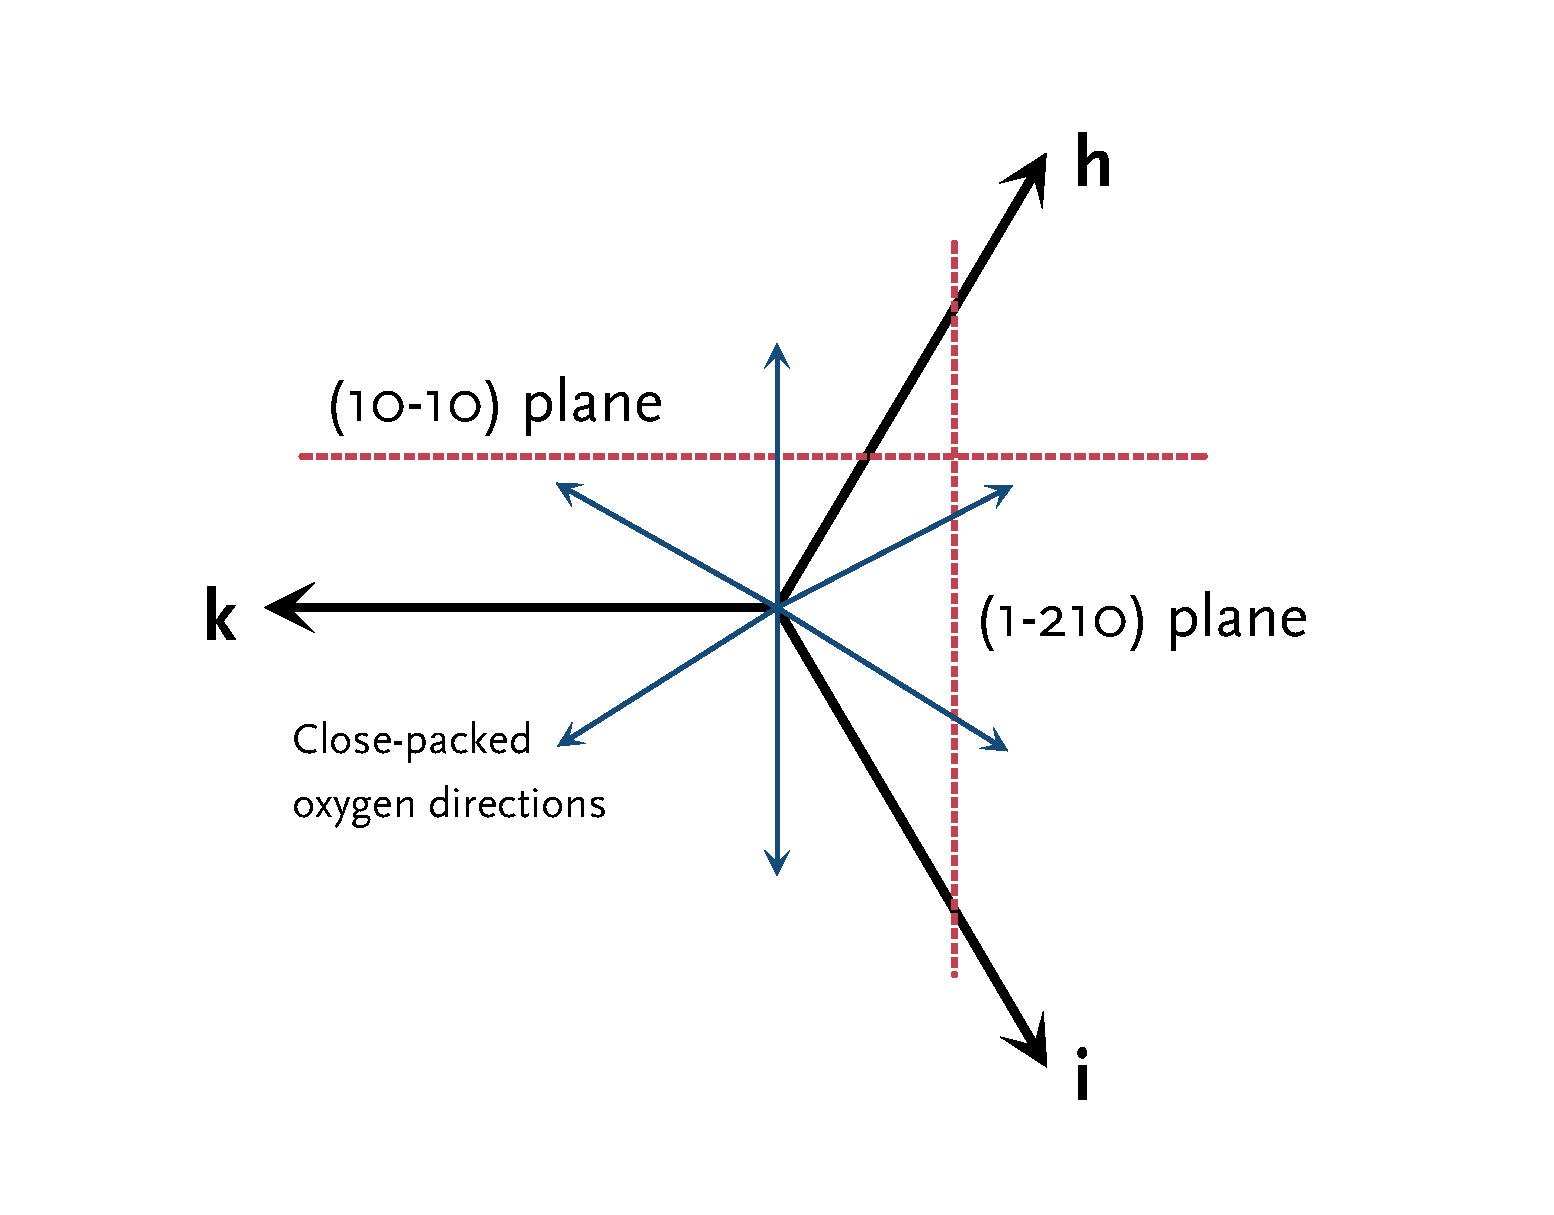
\includegraphics[width=0.6\textwidth]{fe2o3axes.pdf}
\caption[(1\={2}10) and (10\={1}0) planes in relation to in-plane crystal axes]{%
	Schematic showing the (1\={2}10) and (10\={1}0) planes in 
	relation to the in-plane hexagonal crystal axes. Also shown 
	are the close-packed directions of the close packed oxygen 
	network of the basal plane. These close packed directions are 
	located \SI{30}{\degree} from the in-plane crystal axes. The 
	(1\={2}10) planes are perpendicular to the axes of the unit 
	cell, while the (10\={1}0) planes are perpendicular to the 
	close packed directions.
}
\label{fig:fe2o3axes}
\end{center}
\end{figure}
%\sidefigure[(1\={2}10) and (10\={1}0) planes in relation to in-plane crystal axes]{%
%	Schematic showing the (1\={2}10) and (10\={1}0) planes in 
%	relation to the in-plane hexagonal crystal axes. Also shown 
%	are the close-packed directions of the close packed oxygen 
%	network of the basal plane. These close packed directions are 
%	located \SI{30}{\degree} from the in-plane crystal axes. The 
%	(1\={2}10) planes are perpendicular to the axes of the unit 
%	cell, while the (10\={1}0) planes are perpendicular to the 
%	close packed directions.
%	\label{fig:fe2o3axes}
%	}{%
%	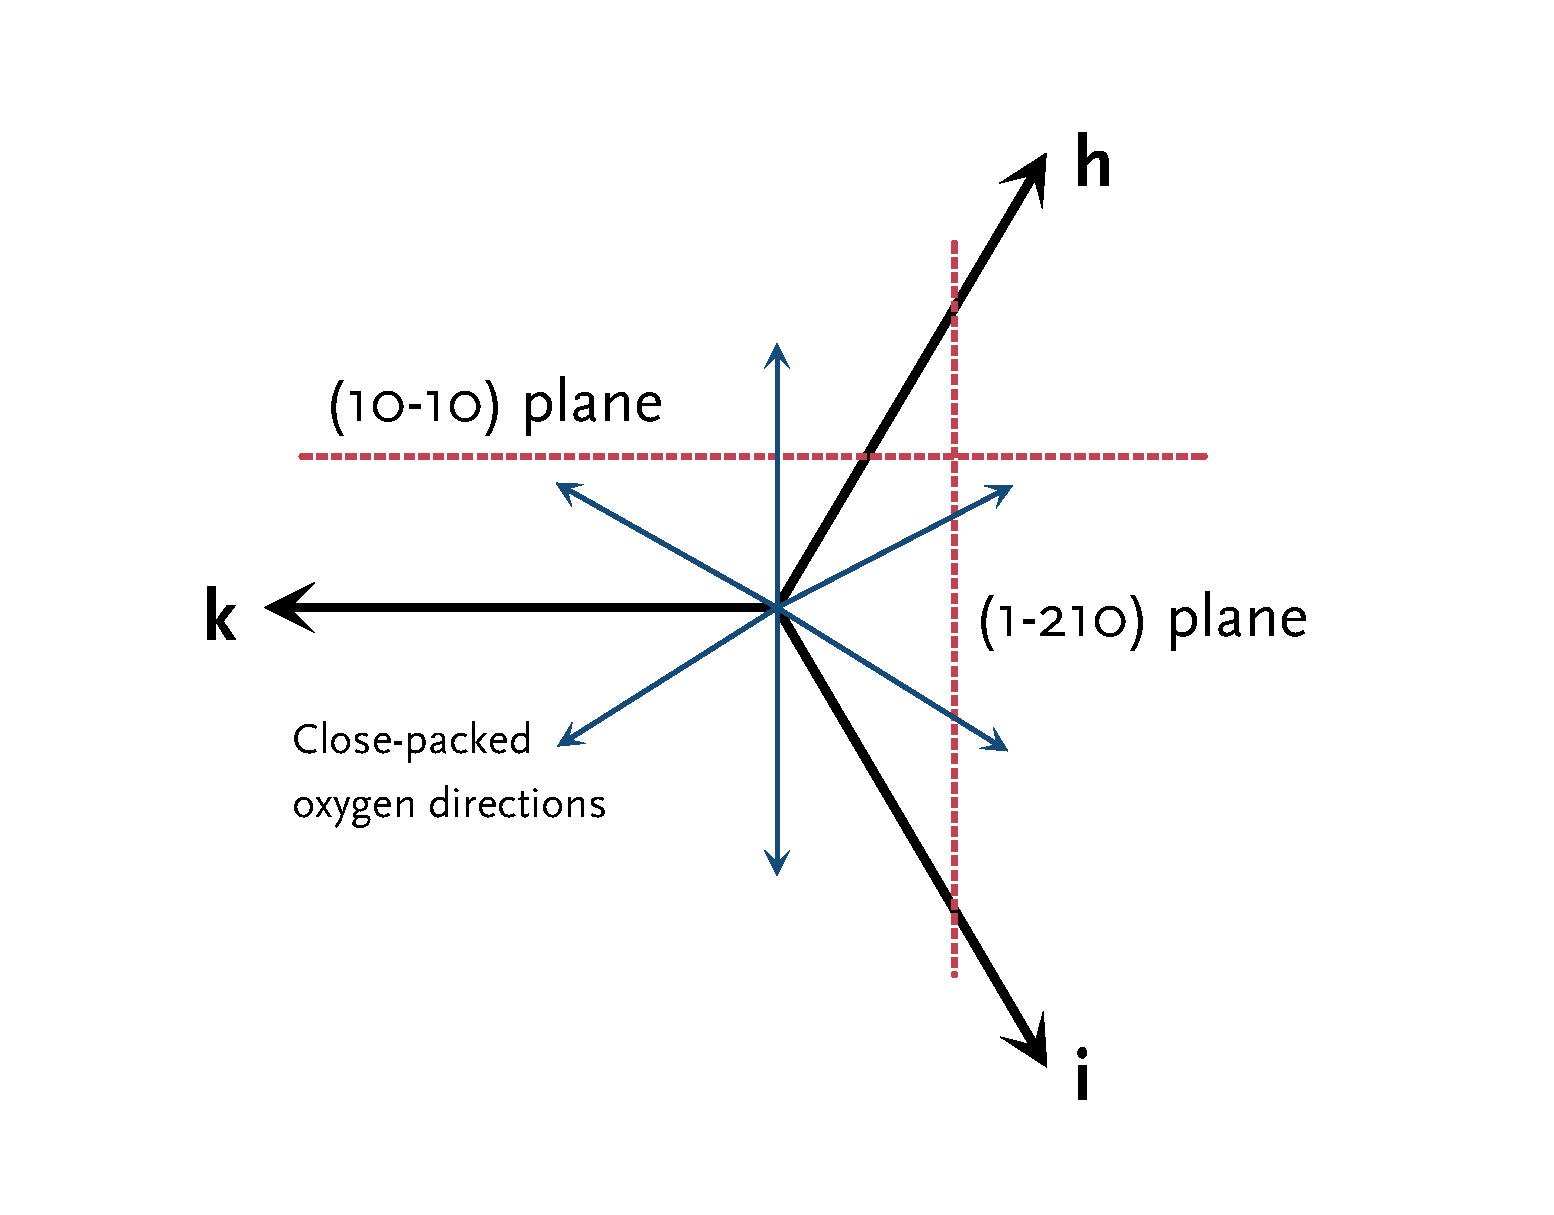
\includegraphics[width=\marginparwidth]{fe2o3axes.pdf}
%}{-20}	
			
The two low-index prismatic orientations  of \ce{Fe2O3} are (in 4-index notation) the
\{1\={2}10\} and the \{10\={1}0\} families. These planes are depicted in
\figureref{fe2o3axes}. Polycrystalline grains near the (1\={2}10) orientation were
significantly more reactive than all other orientations, including the (10\={1}0)
orientation. The data acquired from Kelvin probe force microscopy show that the reactive
orientation are associated with a higher surface potential than the surrounding nonactive
grains. It is logical that grains with a higher surface potential correspond to a higher
reactivity for photochemical reduction reactions, which includes the reduction of aqueous
silver in this work. A more positive potential at the surface would decrease upward or
increase downward band bending at the surface. In this case, reactive grains were an
average of \SI{70}{\milli\volt} more positive than nonreactive grains. 
%The effect of the difference in band bending on photochemical activity is shown
%schematically in the energy level diagram in \figureref{fe2o3bending}.
%\begin{figure}[htbp]
%\begin{center}
%
\includegraphics[width=0.8\textwidth]{fe2o3bending.pdf}
%\caption{Schematic energy level diagram showing the effect of a higher surface potential
%on the band bending and photochemical activity of hematite. The higher surface potential
%decreases upward band bending at the surface of the n-type \ce{Fe2O3}. The reduction in
%upward band bending allows more photogenerated electrons to reach the surface and
%participate in the photochemical reduction of silver ions.}
%\label{fig:fe2o3bending}
%\end{center}
%\end{figure}

An examination of the possible surface terminations of prismatic hematite orientations
gives a possible explanation for the increased reactivity. \figureref{fe2o3terminations}
shows atomic models of the (1\={2}10) and (10\={1}0) planes of \ce{Fe2O3}.
\begin{figure}[htbp]
\begin{center}$
\begin{array}{cc}
\centerline{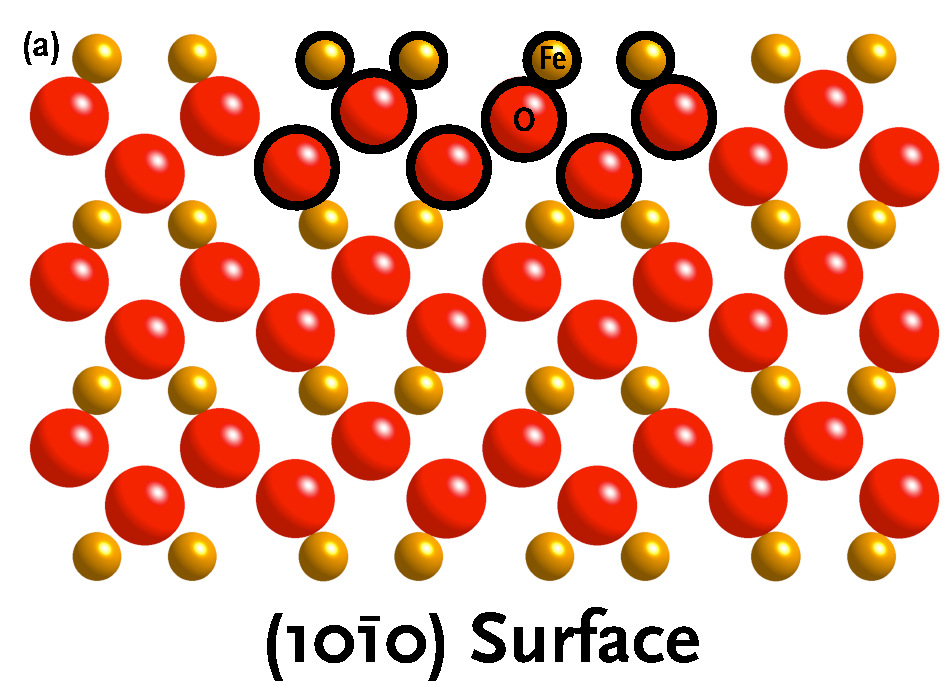
\includegraphics[width=0.75\textwidth]{1010surface.pdf}} \\ 
\centerline{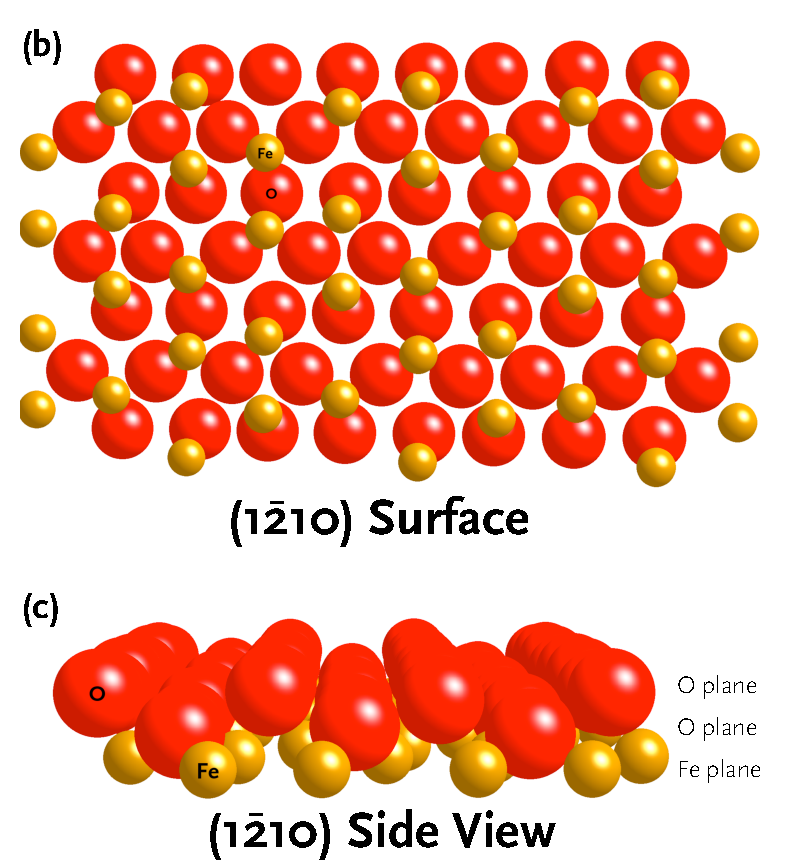
\includegraphics[width=0.75\textwidth]{1210surface.pdf}}
\end{array}$
\caption[Depiction of the (10\={1}0) and (1\={2}10) terminations of hematite]{Depiction of
the (a) (10\={1}0) and (b) (1\={2}10) terminations of hematite. The (10\={1}0) surface is
terminated by a neutral formula unit. Outlined atoms in (a) represent the neutral
repeating \abbr{2D} unit cell. The (1\={2}10) surface is terminated by a polar termination
of either a layer of iron atoms or oxygen atoms. (c) Side view of the (1\={2}10) surface,
showing alternating layers of O or Fe atoms.}
\label{fig:fe2o3terminations}
\end{center}
\end{figure}
The (10\={1}0) is neutral, terminated by a formula unit of \ce{Fe^{3+}} and \ce{O^{2-}}
ions. On the other hand, the (1\={2}10) surface is terminated by alternating layers of
\ce{O^{2-}} and \ce{Fe^{3+}}. For \ce{Fe2O3} films on single crystal substrates presented
in the following chapter, polar surface terminations are present in the more reactive
case. The basal plane is also terminated by polar planes, but as already stated, mobility
along the c-axis is low, which would account for lack of active orientations along this
direction.

\begin{figure}
    \begin{center}
    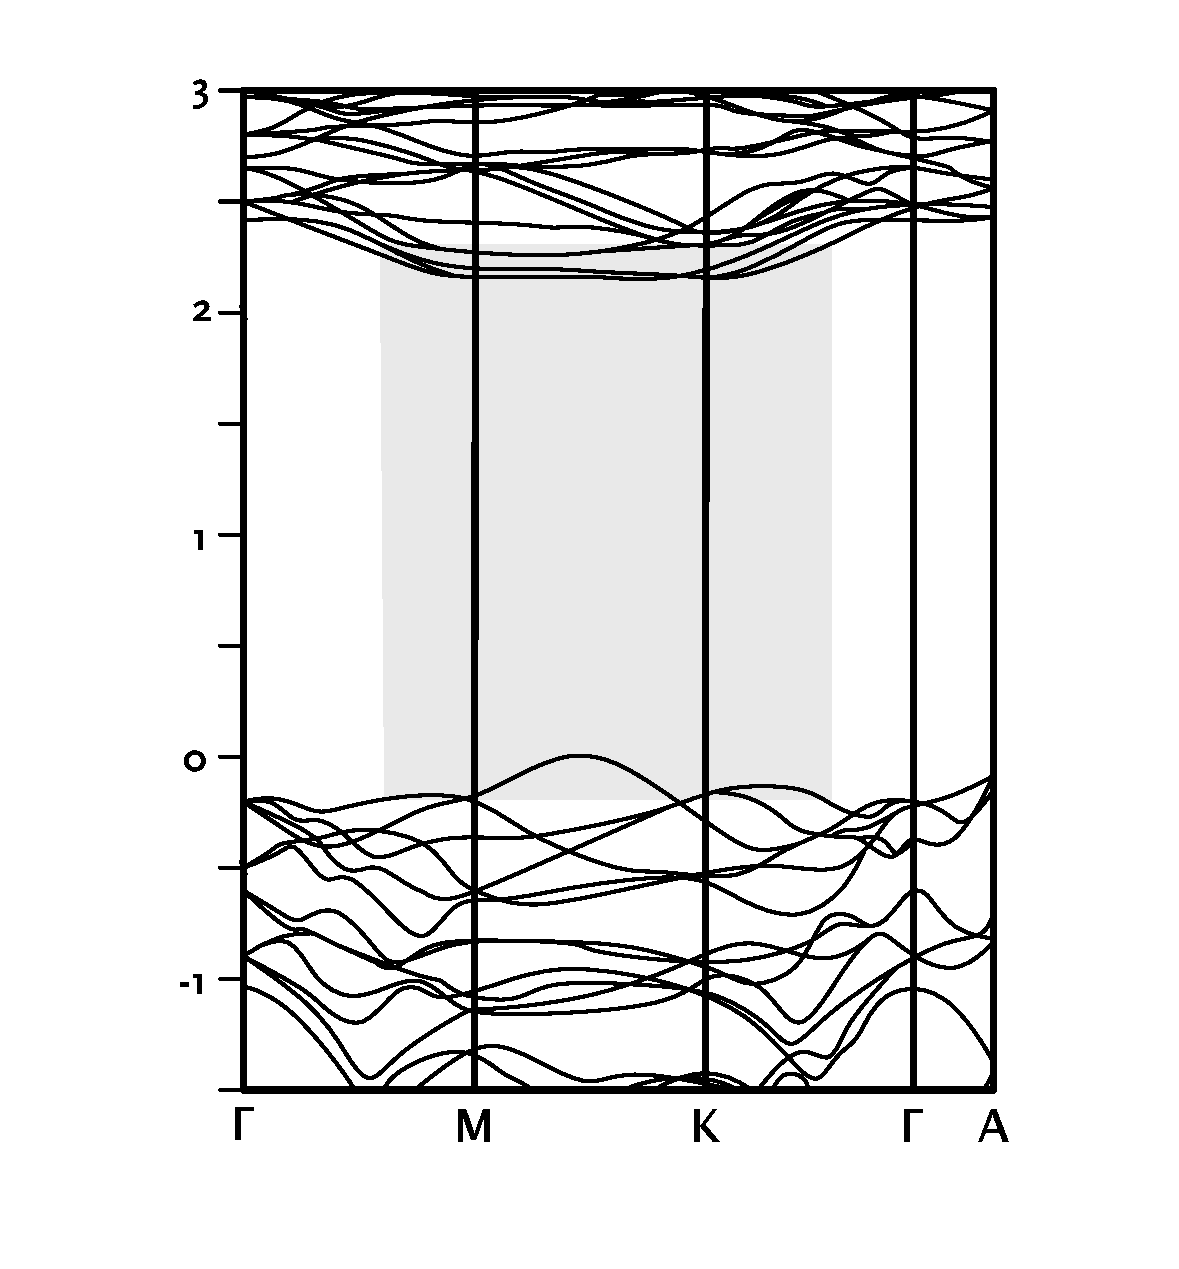
\includegraphics[width=0.6\textwidth]{fe2o3dispersion.pdf}
    \caption[Calculated hematite band electronic band structure]{%
        Calculated hematite band electronic band structure. The bands were reproduced from
        Huda et al.,\cite{Huda:2010kx} but have been rigidly shifted to reflect the experimentally
        observed band gap. The shaded region represents the momentum states where vertical
        transitions are possible with the energy of light from the blue \abbr{LED} used in these
        experiments.}
    \label{fig:fe2o3dispersion}
    \end{center}
\end{figure}
%\sidefigure[Calculated hematite band electronic band structure]{%
%	Calculated hematite band electronic band structure, reproduced from reference
%\citet{Huda:2010kx}.
%	\label{fig:fe2o3dispersion}
%	}{%
%	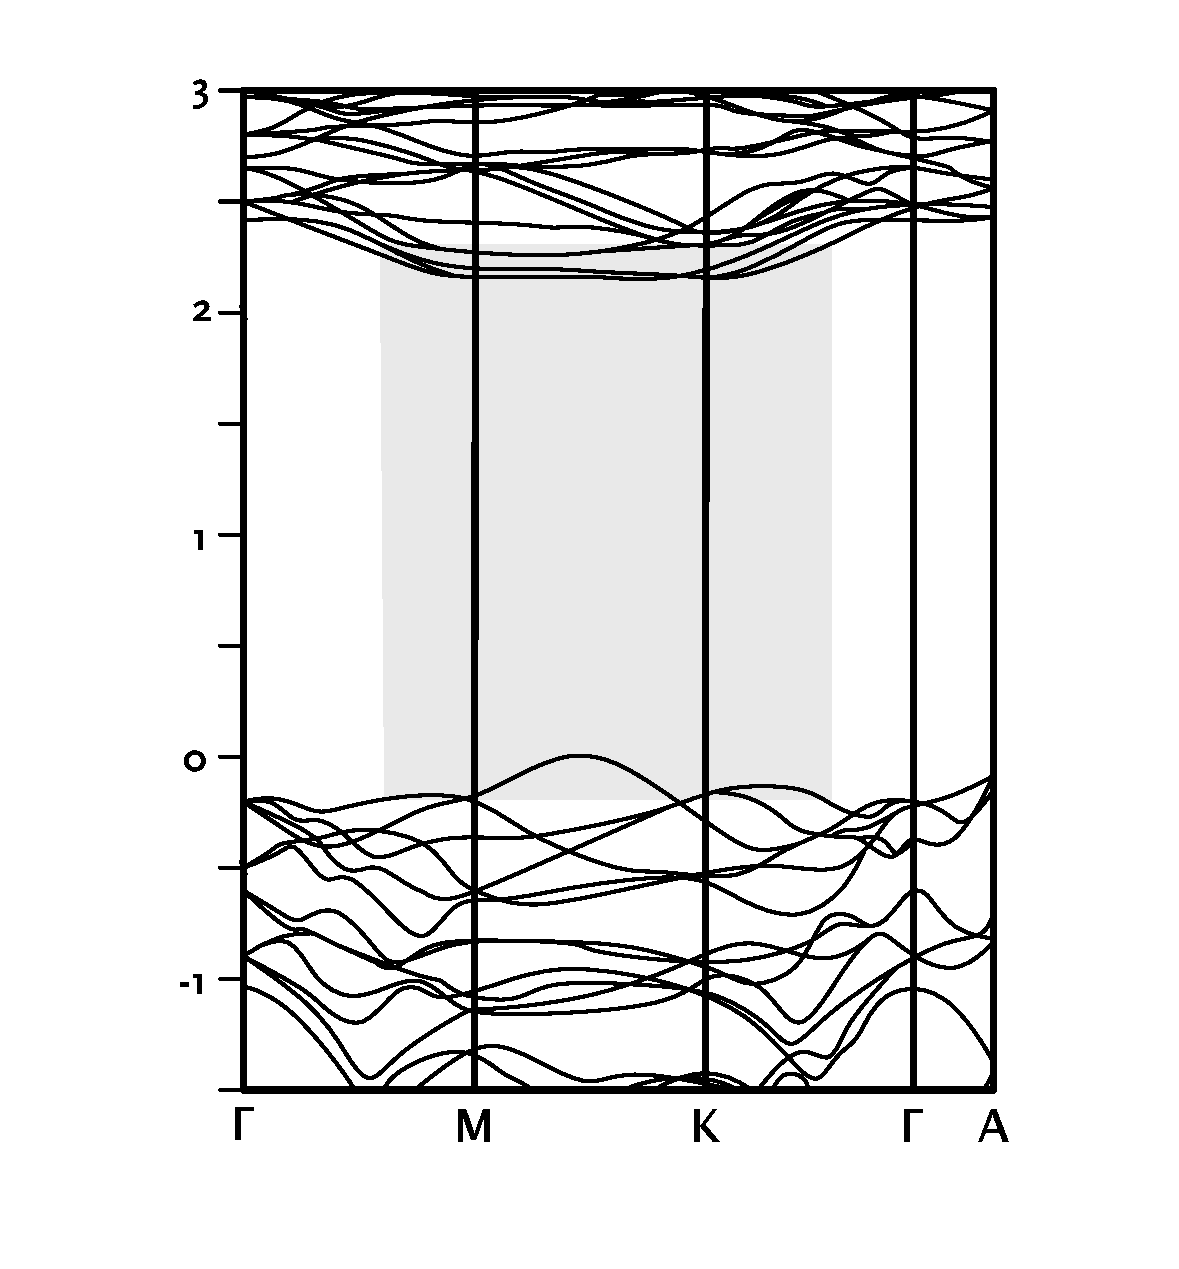
\includegraphics[width=\marginparwidth]{fe2o3dispersion.pdf}
%}{0}	
Giocondi et al.\cite{Giocondi:2007fa} hypothesized that differences in photochemical
reactivity of \ce{SrTiO3} arise from preferred charge carrier generation along certain
crystallographic directions. \figureref{fe2o3dispersion} presents a calculated band
dispersion for hematite \ce{Fe2O3}. For hexagonal crystals, {\textGamma} represents the
center of the Brillouin zone. \textGamma$\rightarrow${\textAlpha} represents charge
carriers generated along the c-axis direction (parallel to the [0001] direction).
\textGamma$\rightarrow${\textMu} represents carriers generated perpendicular to the
(1\={2}10) plane (parallel to a prismatic axis). \textGamma$\rightarrow${\textKappa}
represents the generation of carriers perpendicular to the (10\={1}0) orientation,
traveling in a direction \SI{30}{\degree} offset from a prismatic axis, along a close
packed oxygen direction.

The band structure gives another explanation for the low reactivity of (0001) faces of
bulk hematite. The direct band gap for electrons traveling perpendicular to this face is
on the order of 0.3-0.5 \si{\electronvolt} larger than for electrons traveling toward the
prismatic faces. The larger band gap is expected to result in fewer charge carriers
generated in that direction than for the other faces. This is particularly true in the
case of illumination by the wide spectrum Xe lamp, which generates more low energy photons
than the blue \abbr{LED}. However, the band dispersion shows little difference in the band
gap when comparing the M and K points, which correspond to the (1\={2}10) and (10\={1}0)
zones respectively.
%The \SI{470}{\nano\meter} peak of the blue \abbr{LED} corresponds to a photon energy of
%\SI{2.6}{\electronvolt}, which is of sufficient to generate charge carriers in all
%directions. 



\section{Conclusions and Context}\label{sec:ch9conclusion} 

The (1\={2}10) orientated grains of polycrystalline \ce{Fe2O3} are significantly more
reactive than all other orientations, including other low index prismatic orientations.
Reactive grains correspond to grains with a higher surface potential, as determined
through Kelvin probe force microscopy. The anisotropy in photochemical activity is the
same for reactions performed under wide spectrum light including ultraviolet light as well
as for narrow spectrum visible light from a blue \abbr{LED}. The reactive orientation
corresponds to a prismatic direction terminated by polar surface planes with a significant
number of low energy electrons having momentum in that direction. 

In the context of the other work presented in this document, these results serve to
clarify some of the complicated results presented in later chapters and introduce the
effect of polar surface terminations on photochemical reactivity. This work provides 
information on base reactivity of bulk, polycrystalline hematite. It also correlates
reactivity with grain orientation. These results provide a context for future results. 
For example, for bulk hematite, the c-axis (0001) orientation is consistently not as 
reactive as the (1\={2}10) face, and orientation is not a key factor driving the results 
for films on single crystals presented in \chapterref{single.crystal.reactivity}. Similar 
interpretations can be applied to the results for films on polycrystalline substrates 
presented in \chapterref{polycrystalline.reactivity}. 